\documentclass[border=20pt]{standalone}%book, beamer
%Inicia preámbulo

%\include{tesis}


%\usepackage{fourier}
\usepackage{mathpazo}
\usepackage{antpolt}

% to change the fonts

\usepackage{array}

\usepackage{pdfpages}
\usepackage[utf8]{inputenc}
%\usepackage[numbers]{natbib}
\usepackage[english]{babel}
\usepackage{mathptmx}
\usepackage{amsmath}
\usepackage{graphicx}

\usepackage{xcolor}

%\usepackage[margin=1.5cm]{geometry}
\usepackage{fancyhdr}
\usepackage{parskip}
\usepackage[colorlinks=false]{hyperref}
\usepackage{amsmath}
\usepackage{amsmath,amsfonts}
\usepackage{amssymb}
\usepackage{mathrsfs}
\usepackage{siunitx}
%\usepackage[usenames]{color}
\usepackage{multirow} % para las tablas
%\usepackage[spanish,es-tabla]{babel}
\usepackage{hieroglf}
\usepackage{caption}
\usepackage{subcaption}
\usepackage{wrapfig}
\usepackage{booktabs}
%\usepackage{slashbox}
%\usepackage{tcolorbox}
\usepackage{multicol}
\usepackage{fontenc}
%\usepackage{tgbonum}

\usepackage{float}
\usepackage{booktabs}
\usepackage{indentfirst}


\usepackage{indentfirst}
\usepackage{tabularray}

\usepackage{lscape}

\usepackage{listings}
\usepackage{appendix}

\usepackage{multicol}
\setlength{\columnsep}{1cm}

\usepackage{nameref}

\usepackage{tikz}
\usetikzlibrary{datavisualization.formats.functions} % LaTeX and plain TeX

\usetikzlibrary[datavisualization]
\usepackage{pgfplots}
\pgfplotsset{compat=1.18}

\usepackage[siunitx, RPvoltages,american resistor]{circuitikz}


%\usetikzlibrary {circuits.ee.IEC} 
\newcommand*{\TickSize}{2pt}%

\ctikzset{quadpoles/transformer core/height=3}
\usepgfplotslibrary{fillbetween}
\author{Mario Sepúlveda-Hernández}
\date{\today}
\title{Full wave rectifier}
\begin{document}
	
	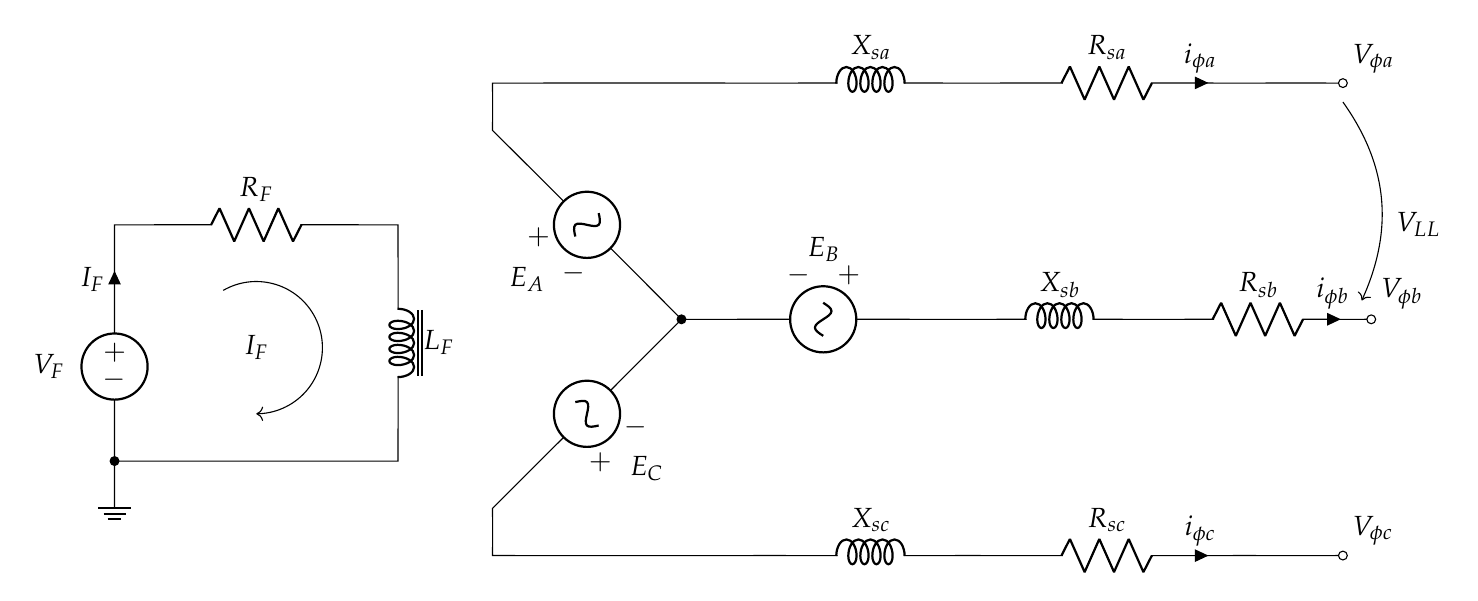
\begin{tikzpicture}[american,scale=1.2]
		\draw (0,-1) node[tlground]{} to [V=$V_{F}$,i=$I_{F}$] (0,2) 
		to [american resistor=$R_{F}$] (3,2)
		to [cute inductor=$L_{F}$,name=myL,label distance=2.4pt] (3,-0.5)
		to [short,-*] (0,-0.5);
		\draw[thick, double] (myL.core west) -- (myL.core east);
		\draw (6,1) to [sV=$E_{B}$,*-] (9,1)
		to [cute inductor=$X_{sb}$] (11,1)
		to [resistor=$R_{sb}$,i=$i_{\phi b}$]  (13.2,1)
		to [short,-o] (13.3,1) node[anchor=south west]{$V_{\phi b}$};
		\draw (6,1) to [sV=$E_{A}$] (4,3)
		to [short] (4,3.5)
		to [short] (7,3.5)
		to [cute inductor=$X_{sa}$] (9,3.5)
		to [resistor=$R_{sa}$,i=$i_{\phi a}$] (12,3.5)
		to [short,-o] (13,3.5) node[anchor=south west]{$V_{\phi a}$};
		\draw[->] (13,3.3) to[bend left] (13.2,1.2)
		node at(13.8,2){$V_{LL}$};
		\draw (6,1) to [sV=$E_{C}$] (4,-1)
		to [short] (4,-1.5)
		to [short] (7,-1.5)
		to [cute inductor=$X_{sc}$] (9,-1.5)
		to [resistor=$R_{sc}$,i=$i_{\phi c}$](12,-1.5)
		to [short,-o] (13,-1.5) node[anchor=south west]{$V_{\phi c}$};
		\draw[->,shift={(1.5,0.7)}] (120:.7cm) arc (120:-90:.7cm) node at(0,0){$I_{F}$};
	\end{tikzpicture}
	
\end{document}